
%%% Variables de frecuencia por cada base de datos. 
\newcommand{\acm}{518}
\newcommand{\ieee}{0}
\newcommand{\sd}{120}
\newcommand{\spr}{209}
\newcommand{\tf}{0}
\newcommand{\tot}{847}
%%% Variables de contrubución porcetual
\newcommand{\acmp}{\fpeval{round(\acm*100/\tot,2)}}
\newcommand{\ieeep}{\fpeval{round(\ieee*100/\tot,2)}}
\newcommand{\sdp}{\fpeval{round(\sd*100/\tot,2)}}
\newcommand{\sprp}{\fpeval{round(\spr*100/\tot,2)}}
\newcommand{\tfp}{\fpeval{round(\tf*100/\tot,2)}}

%%%%% ------------------------------------------------

%%% Variables de frecuencia por cada base de datos. 
\newcommand{\iacm}{315}
\newcommand{\iieee}{0}
\newcommand{\isd}{101}
\newcommand{\ispr}{63}
\newcommand{\itf}{0}
\newcommand{\itot}{479}
%%% Variables de contribución porcentual
\newcommand{\iacmp}{\fpeval{round(\iacm*100/\itot,2)}}
\newcommand{\iieeep}{\fpeval{round(\iieee*100/\itot,2)}}
\newcommand{\isdp}{\fpeval{round(\isd*100/\itot,2)}}
\newcommand{\isprp}{\fpeval{round(\ispr*100/\itot,2)}}
\newcommand{\itfp}{\fpeval{round(\itf*100/\itot,2)}}

%Cantidad de estudios excluídos por ser duplicados
\newcommand{\numEstEx}{3}

%Cantidad de estudios luego de depuración = (estudios totales luego de exclusión - estudios duplicados)
\newcommand{\depTot}{\fpeval{\itot-\numEstEx}}

%Cantidad de estudios depurados por el screening
\newcommand{\screen}{377}
%Cantidad de estudios totales luego del screening
\newcommand{\screenTot}{\fpeval{\depTot-\screen}}

%sub-subseccion 4.2.2
\subsubsection{Estrategia de Búsqueda 1: Bases de Datos}

Esta estrategia comprende dos componentes. El primer componente se denomina ``Identificación de estudios''. Se enfoca en establecer las palabras clave para construir las cadenas de búsqueda que permitan completar las consultas en las bibliotecas digitales. El segundo componente se denomina ``Selección de estudios''. Se enfoca en aplicar varios criterios para refinar los resultados de búsqueda de estudios y seleccionar aquellos con el valor más significativo para el SMS.\@

\bolditalic{Identificación de estudios}: con el fin de asegurar la viabilidad del SMS y por consenso de los autores, se decidió limitar el número de bases de datos a cinco, incluyendo ACM, IEEE Xplore, Springer, ScienceDirect, Taylor \& Francis. En esta parte del proceso, es necesario establecer las palabras clave utilizadas posteriormente en las cadenas de búsqueda de cada una de las bases de datos. Nuevamente utilizamos el modelo PICOC como guía metodológica para identificar términos o frases clave que cumplan este propósito. Refinamos estos términos incluyendo sinónimos (Ver Tabla \ref{table:picoc_keywords}).

% -------- Tabla : Palabras clave del modelo PICOC. ------------
\begin{table}[htbp]
	\centering
	\caption{Palabras clave identificadas usando el modelo PICOC}
	\label{table:picoc_keywords}
	\renewcommand{\arraystretch}{1}  % Increase row height globally
	\begin{tabular}{p{1.8cm}p{6cm}}
		\toprule
		\textbf{Componente}              & \textbf{Palabras clave}                                                                                                                                                                                                                                                                 \\
		\midrule
		\textbf{Población}               & Universos, HTCondor, Computación distribuida y paralela, HTC, Desarrollo de Software, Virtualización y microservicios, Redes de computadoras, Infraestructura computacional, Inteligencia artificial, Análisis de datos, Pensamiento computacional, Investigación, Docencia, Extensión. \\
		\addlinespace[0.8em]
		\textbf{Intervención}            & Identificación y clasificación.                                                                                                                                                                                                                                                         \\
		\addlinespace[0.8em]
		\textbf{Criterios de aceptación} &
		Casos de proyecto documentados, cumplimiento de criterios de inclusión y exclusión y aparición en bases de datos seleccionadas.                                                                                                                                                                                            \\
		\addlinespace[0.8em]
		\textbf{Salidas}                 & Taxonomía que organiza los trabajos relacionados con la población.                                                                                                                                                                                                                      \\
		\addlinespace[0.8em]
		\textbf{Contexto}                & Universos HTCondor, dominios de computación distribuida y paralela, funciones sustantivas universitarias , investigación, docencia, extensión.                                                                                                                    \\
		\bottomrule
	\end{tabular}
\end{table}
% --------------------------------------------------------------



Las palabras clave principales que seleccionamos fueron \textit{HTCondor, HTC, Universe, Project, Research}. Para ampliar la perspectiva de investigación, utilizamos el operador booleano ``OR'' para agregar sinónimos a las palabras clave principales.
Finalmente, el conjunto de palabras clave seleccionadas para la construcción de la cadena de búsqueda se encuentran en la Tabla \ref{table:database_search_keywords}.



% -------- Tabla : Palabras clave para búsqueda en base de datos . ------------
\begin{table}[htbp]
	\centering
	\caption{Palabras clave para búsqueda en base de datos}
	\label{table:database_search_keywords}
	\renewcommand{\arraystretch}{1}  % Increase row height globally
	\begin{tabular}{p{1.4cm}p{6.4cm}}
		\toprule
		\textbf{Palabra}  & \textbf{Sinónimos y conceptos relacionados}                \\
		\midrule
		\textbf{HTCondor} & Condor                                                     \\
		\addlinespace[0.8em]
		\textbf{HTC}      & HPC, High Throughput Computing, High Performance Computing \\
		\addlinespace[0.8em]
		\textbf{Universe} & Execution Environment                                      \\
		\addlinespace[0.8em]
		\textbf{Project}  & Work                                                       \\
		\addlinespace[0.8em]
		\textbf{Research} & Teaching, Industry                                         \\
		\bottomrule
	\end{tabular}
\end{table}
% --------------------------------------------------------------





% --------------- Tabla CADENAS DE Búsqueda-----------------------------------------
% -------- Tabla : Cadenas de búsqueda por base de datos ------------
\begin{table*}[htbp]
	\centering
	\caption{Cadenas de búsqueda utilizadas en las bases de datos}
	\label{table:cadenas_de_busqueda}
	\renewcommand{\arraystretch}{1}  % Increase row height globally
	\begin{tabular}{p{3.2cm}p{11cm}p{2.5cm}}
		\toprule
		\textbf{Base de Datos}            & \textbf{Cadena de Búsqueda}                                                                                                                                                                                        & \textbf{Campos}  \\
		\midrule
		\textbf{ACM Full Text Collection} & ((HTCondor OR Condor) AND (HTC OR ``High Throughput Computin'' OR HPC OR ``High Performance Computing'') AND (Universe OR ``Execution Environment'') AND (Project OR Work) AND (Research OR Teaching OR Industry)) & Todos los campos \\
		\addlinespace[0.8em]
		\textbf{IEEE Xplore}              & (HTCondor OR Condor) AND (HTC OR (High Throughput Computing)) AND (Universe OR (Runtime Environment)) AND (Research OR Teaching OR Industry)                                                                       & Todos los campos \\
		\addlinespace[0.8em]
		\textbf{Springer}                 & ((HTCondor | Condor) + (HTC | ``High Throughput Computing'' | HPC | ``High Performance Computing'') + (Universe | ``Execution Environment'') + (Project | Work) + (Research | Teaching | Industry))                & Todos los campos \\
		\addlinespace[0.8em]
		\textbf{ScienceDirect}            & (HTCondor OR Condor) (HTC OR ``High Throughput Computing'' OR HPC OR ``High Performance Computing'') (Universe OR ``Execution Environment'') (Project OR Work) (Research OR Teaching OR Industry)                  & Todos los campos \\
		\addlinespace[0.8em]
		\textbf{Taylor \& Francis}        & (HTCondor OR Condor) AND (HTC OR (High Throughput Computing)) AND (Universe OR (Runtime Environment)) AND (Research OR Teaching OR Industry)                                                                       & Todos los campos \\
		\bottomrule
	\end{tabular}
\end{table*}
% --------------------------------------------------------------





Para dirigir la investigación hacia la intersección de estos dos grupos de términos, se utilizó el operador booleano ``AND''. Una vez que identificamos las palabras clave, continuamos construyendo las cadenas de búsqueda para las bibliotecas digitales utilizando un proceso iterativo. La construcción iterativa de las cadenas de búsqueda consiste en realizar un proceso heurístico con las palabras clave, sinónimos y conceptos relacionados mediante el uso de disyunciones y conjunciones que se ajustan a las reglas sintácticas de cada base de datos considerada en la búsqueda automática. Por lo tanto, estas cadenas varían según las características y funciones de cada base de datos. Ver Tabla \ref{table:cadenas_de_busqueda}.

Después de construidas las cadenas de búsqueda, estas fueron enviadas a cada motor de base de datos. La Tabla \ref{table:search_results} muestra el conjunto de resultados obtenidos. Identificamos un total de 847 estudios preliminarmente, siendo ACM la mayor contribuidora, entregando la mayor cantidad de resultados respecto a las demás bases de datos con el \acmp\% de los resultados.

% -------- Tabla : Resultados de las cadenas de búsqueda ------------


\begin{table*}[htbp]
	\centering
	\caption{Resultados de las cadenas de búsqueda}
	\label{table:search_results}
	\renewcommand{\arraystretch}{1}  % Increase row height globally
	\begin{tabular}{p{4.8cm}p{1.7cm}p{1.7cm}p{1.7cm}p{1.7cm}p{2cm}p{1.4cm}}
		\toprule
		\textbf{Criterios}                                        & \textbf{ACM} & \textbf{IEEE} & \textbf{ScienceDirect} & \textbf{Springer} & \textbf{Taylor\&Francis} & \textbf{Total} \\
		\midrule
		\textbf{Cadena de búsqueda con palabras clave únicamente} & \acm{}       & \ieee{}       & \sd{}                  & \spr{}            & \tf{}                    & \tot{}         \\
		\addlinespace[0.8em]
		\textbf{Contribución porcentual}                          & \acmp{}\%    & \ieeep{}\%    & \sdp{}\%               & \sprp{}\%         & \tfp{}\%                 & 100\%          \\
		\bottomrule
	\end{tabular}
\end{table*}
% --------------------------------------------------------------




\bolditalic{Selección de estudios}: para refinar los resultados obtenidos hasta este punto, aplicamos los criterios de inclusión y exclusión definidos en la fase de planificación. La Tabla \ref{table:search_results_exclusion} muestra los resultados de este paso. Después de aplicado dicho filtro, el número total de estudios obtenido fue \itot. Según las diferentes bases de datos consultadas, ACM continúa teniendo la contribución más considerable, con el \iacmp\% de los estudios.




%% Aplicando exclusion duplicada

De los \itot{} estudios seleccionados, se aplicó la exclusión de tres estudios dado que estos eran duplicados. Después de esta depuración, los estudios totales fueron \depTot{}. A partir de este nuevo conjunto de datos, se realizó una revisión con el nombre de  \bolditalic{screening}, este procedimiento consiste en verificar el título, resumen y palabras clave de cada estudio para determinar si estos se encuentran circunscritos en el contexto de la investigación, es decir, si están alineados a los objetivos propuestos para el SMS. El proceso de \textit{screening} nos permitió descartar \screen{} estudios dado que algunos de ellos hacían referencia a disciplinas académicas diferentes y otros no estaban alineados con los objetivos de investigación planteados.

Por lo tanto, concluimos la primera estrategia de búsqueda con un total de \screenTot{} estudios seleccionados. La Figura \ref{fig:overview} muestra una visión general de las actividades y resultados obtenidos en la estrategia de búsqueda 1.

\begin{figure}[htbp]
	\centering
	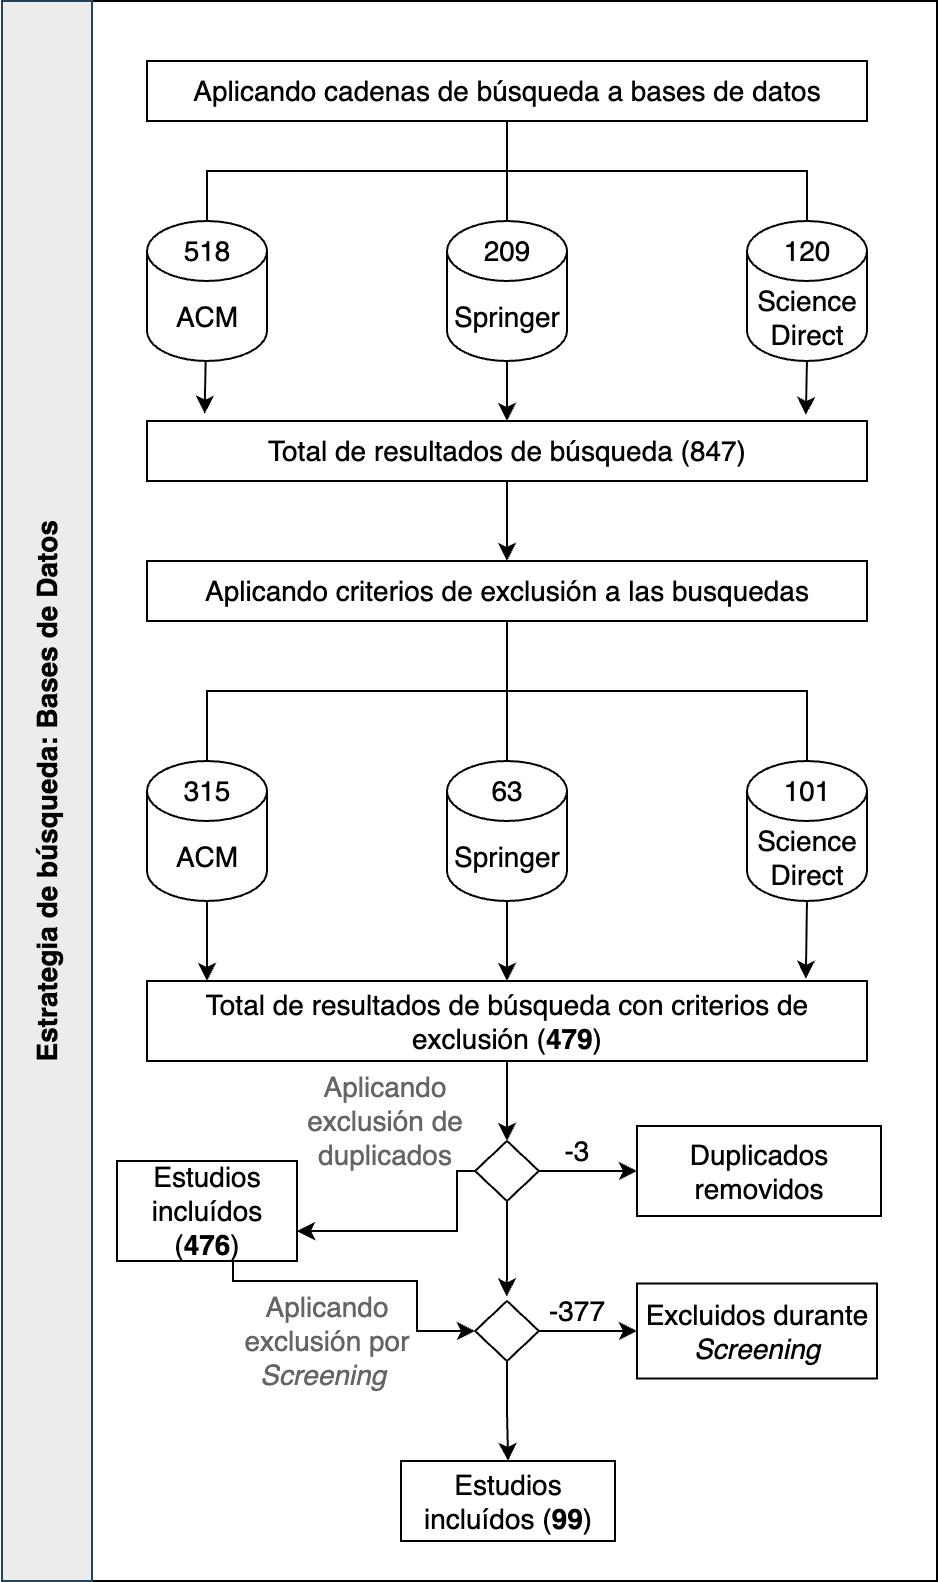
\includegraphics[scale=0.25]{resources/figures/overview.png}
	\caption{Vista general de las actividades y resultados obtenidos en la estrategia de búsqueda por bases de datos}
	\label{fig:overview}
\end{figure}


\begin{table*}[htbp]
	\centering
	\caption{Resultados de las cadenas de búsqueda con criterios de exclusión}
	\label{table:search_results_exclusion}
	\begin{tabular}{p{4.8cm}p{1.7cm}p{1.7cm}p{1.7cm}p{1.7cm}p{2cm}p{1.4cm}}
		\toprule
		\textbf{Criterios}                                        & \textbf{ACM} & \textbf{IEEE} & \textbf{ScienceDirect} & \textbf{Springer} & \textbf{Taylor \& Francis} & \textbf{Total} \\
		\midrule
		\textbf{Cadena de búsqueda con palabras clave únicamente} & \iacm{}      & \iieee{}      & \isd{}                 & \ispr{}           & \itf{}                     & \itot{}        \\
		\addlinespace[0.8em]
		\textbf{Contribución porcentual}                          & \iacmp{}\%   & \iieeep{}\%   & \isdp{}\%              & \isprp{}\%        & \itfp{}\%                  & 100\%          \\
		\bottomrule
	\end{tabular}
\end{table*}
% --------------------------------------------------------------

